\documentclass[../cours_3e.tex]{subfiles}
\begin{document}
\setcounter{chapter}{11}
\chapter{Les fondements de la géométrie plane}
\label{ch:geometrie}
\begin{objectif}
Maîtriser les angles, triangles, médiatrices et quadrilatères ; construire une figure et justifier ses propriétés. Ces acquis du collège sont indispensables aux chapitres suivants.
\end{objectif}
\section{Objets, codage et points de départ}
Une droite est illimitée ; un segment est limité par ses extrémités. Deux droites distinctes du plan sont parallèles si elles ne se coupent pas. Elles sont perpendiculaires si elles forment un angle droit. Le cercle de centre $O$ et de rayon $r>0$ est l'ensemble des points à distance $r$ de $O$ ; le disque comprend aussi l'intérieur.

Une figure codée indique les données : traits identiques pour des longueurs égales, arcs identiques pour des angles égaux, petit carré pour un angle droit. Un dessin à main levée peut être exact dans ses données même si les proportions visuelles sont approximatives.

\admis{Nous travaillons dans le plan euclidien : deux points distincts définissent une droite ; par un point extérieur passe une unique parallèle à une droite donnée ; les déplacements rigides conservent les longueurs et les angles ; le segment est le plus court chemin entre ses extrémités. La caractérisation des parallèles par les angles correspondants est une propriété de base de ce cadre, non reconstruite à partir d'une axiomatique complète.}
\section{Angles et parallélisme}
Un angle droit mesure $90\degre$, un angle plat $180\degre$, un tour $360\degre$. Deux angles complémentaires ont une somme de $90\degre$ ; deux angles supplémentaires ont une somme de $180\degre$.
\begin{propriete}
Deux angles opposés par le sommet sont égaux. Deux parallèles coupées par une sécante déterminent des angles correspondants égaux et des angles alternes-internes égaux. Réciproquement, une telle égalité permet de prouver le parallélisme.
\end{propriete}
\begin{demonstration}
Si deux angles opposés par le sommet sont $\alpha$ et $\gamma$, un angle adjacent $\beta$ vérifie $\alpha+\beta=180\degre$ et $\gamma+\beta=180\degre$. En soustrayant $\beta$, $\alpha=\gamma$.
L'égalité des angles correspondants pour des parallèles est prise comme base euclidienne. Celle des alternes-internes en découle avec l'égalité des angles opposés par le sommet. Les réciproques se ramènent à l'unicité de la parallèle passant par un point : tracer cette parallèle crée l'angle requis ; une autre droite formant le même angle et du même côté se confond avec elle.
\end{demonstration}
\begin{center}
\begin{tikzpicture}[scale=.85]
\draw(-3,0)--(3,0)node[right]{$d$};
\draw(-3,2)--(3,2)node[right]{$d'$};
\draw(-2,-1)--(2,3);
\draw[accent,thick](.6,2)arc(180:225:.4);
\draw[accent,thick](-.6,0)arc(0:45:.4);
\node[accent]at(.25,1.65){$\alpha$};
\node[accent]at(-.25,.35){$\alpha$};
\end{tikzpicture}
\end{center}
Dans une rédaction, nommer les trois points de chaque angle évite de confondre une paire d'angles avec une autre.
\section{Triangles : angles, existence et hauteurs}
\begin{theoreme}
La somme des angles d'un triangle vaut $180\degre$.
\end{theoreme}
\begin{demonstration}
Dans le triangle $ABC$, tracer par $A$ la parallèle à $(BC)$. Les angles qu'elle forme avec $(AB)$ et $(AC)$ reproduisent les angles en $B$ et $C$ par alternance interne. Avec l'angle $\widehat{BAC}$, ils forment un angle plat. Leur somme est donc $180\degre$.
\end{demonstration}
\begin{center}
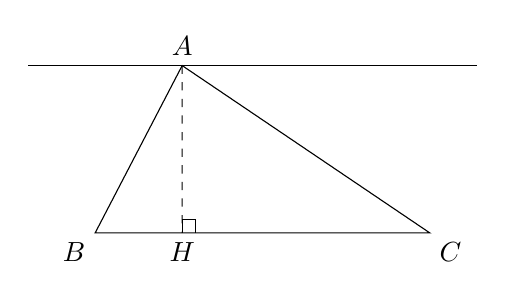
\begin{tikzpicture}[scale=.85]
\coordinate(A)at(1.3,2.5);\coordinate(B)at(0,0);\coordinate(C)at(5,0);
\draw(-1,2.5)--(5.7,2.5);\draw(A)--(B)--(C)--cycle;
\foreach \p/\pos in {A/above,B/below left,C/below right}{\node[\pos]at(\p){$\p$};}
\draw[dashed](A)--(1.3,0)node[below]{$H$};
\draw(1.3,0)--(1.3,.2)--(1.5,.2)--(1.5,0);
\end{tikzpicture}
\end{center}
\begin{definition}
Une hauteur d'un triangle est une droite passant par un sommet et perpendiculaire à la droite du côté opposé. Sa longueur associée est la distance du sommet à cette droite. Le pied peut être à l'extérieur du triangle.
\end{definition}
\begin{propriete}[Inégalité triangulaire]
Dans un triangle non aplati, chaque côté est strictement plus court que la somme des deux autres. Pour trois points quelconques, $AB+BC\geq AC$, avec égalité lorsque $B\in[AC]$.
\end{propriete}
\begin{justification}
Aller directement de $A$ à $C$ est le plus court chemin. Passer par $B$ est plus long sauf si $B$ est sur le segment direct. Ce principe de distance est l'un des points de départ admis plus haut.
\end{justification}
Pour construire un triangle de côtés $a\leq b\leq c$, vérifier $a+b>c$. Avec $2,3,6$, il est impossible ; avec $2,3,5$, il est aplati ; avec $3,4,5$, il existe.
\section{Triangles égaux et constructions}
\begin{definition}
Deux triangles sont \textbf{égaux} ou \textbf{superposables} si l'on peut faire coïncider leurs sommets par un déplacement rigide, éventuellement après retournement.
\end{definition}
\begin{propriete}
Deux triangles sont égaux si l'on connaît respectivement :
\begin{itemize}
\item les trois côtés égaux (CCC) ;
\item deux côtés et l'angle \emph{compris entre eux} égaux (CAC) ;
\item un côté et ses deux angles adjacents égaux (ACA).
\end{itemize}
\end{propriete}
\begin{demonstration}
Pour CCC, superposer un côté. Le troisième sommet appartient à deux cercles de centres aux extrémités du côté et de rayons fixés. Les deux choix possibles sont symétriques par rapport au côté : ils donnent des triangles superposables.
Pour CAC, superposer le sommet et les deux directions déterminées par l'angle ; les longueurs fixent les deux autres sommets.
Pour ACA, superposer le côté ; les deux demi-droites déterminées par les angles fixent leur point d'intersection. Ces arguments s'appuient sur les propriétés élémentaires des constructions à la règle et au compas.
\end{demonstration}
Pour construire un triangle de côtés $4$, $5$ et $6\unite{cm}$ : tracer le côté de $6\unite{cm}$, puis les cercles de rayons $4$ et $5\unite{cm}$ aux extrémités. Une intersection donne le troisième sommet.
\begin{attention}
Deux côtés et un angle non compris ne suffisent pas toujours. Deux triangles ayant les mêmes angles peuvent avoir des tailles différentes : ils sont semblables, pas forcément égaux.
\end{attention}
\section{Isocèle, équilatéral et médiatrice}
\begin{definition}
Un triangle isocèle possède deux côtés égaux. Un triangle équilatéral en possède trois. La médiatrice d'un segment est la droite perpendiculaire à ce segment passant par son milieu.
\end{definition}
\begin{propriete}
Dans un triangle isocèle, les angles à la base sont égaux. Un triangle équilatéral a trois angles de $60\degre$. Réciproquement, deux angles égaux dans un triangle sont opposés à deux côtés égaux.
\end{propriete}
\begin{demonstration}
Si $AB=AC$, soit $I$ le milieu de $[BC]$. Les triangles $ABI$ et $ACI$ sont égaux par CCC : ils ont $AB=AC$, $BI=CI$ et $AI$ commun. Les angles à la base sont donc égaux. Dans l'équilatéral, appliquer ce résultat à plusieurs sommets donne trois angles égaux ; leur somme $180\degre$ impose $60\degre$ chacun.
Pour la réciproque, comparer $ABC$ et $ACB$ : le côté $BC$ est le même et les deux angles adjacents sont égaux. Le critère ACA donne $AB=AC$.
\end{demonstration}
\begin{theoreme}[Médiatrice et distances]
Un point $M$ appartient à la médiatrice de $[AB]$ si et seulement si $MA=MB$.
\end{theoreme}
\begin{demonstration}
Soit $I$ le milieu de $[AB]$. Si $M$ est sur la médiatrice, les triangles $MIA$ et $MIB$ sont égaux par CAC (côté $MI$ commun, $IA=IB$, angles droits), donc $MA=MB$. Réciproquement, si $MA=MB$ et $M\ne I$, ces triangles sont égaux par CCC ; leurs angles en $I$ sont égaux et supplémentaires, donc droits. Ainsi $(MI)$ est la médiatrice. Le point $I$ lui-même satisfait aussi la propriété.
\end{demonstration}
\begin{methode}[Construire une médiatrice]
Tracer deux arcs de même rayon, supérieur à la moitié de $AB$, de centres $A$ et $B$. Relier leurs deux intersections. Chacune est à égale distance de $A$ et $B$, donc la droite est la médiatrice.
\end{methode}
Les médiatrices de deux côtés d'un triangle non aplati se coupent en un point $O$. Comme $OA=OB$ et $OB=OC$, on a aussi $OA=OC$ : la troisième médiatrice passe par $O$. Le cercle de centre $O$ et de rayon $OA$ passe par les trois sommets ; c'est le cercle circonscrit.
\section{Parallélogrammes et cas particuliers}
\begin{definition}
Un parallélogramme est un quadrilatère dont les côtés opposés sont parallèles. Un rectangle a quatre angles droits. Un losange a quatre côtés égaux. Un carré est à la fois rectangle et losange.
\end{definition}
\begin{theoreme}[Caractérisation]
Un quadrilatère non aplati est un parallélogramme si et seulement si ses diagonales ont le même milieu.
\end{theoreme}
\begin{demonstration}
Dans un parallélogramme $ABCD$, la diagonale $AC$ détermine deux triangles égaux par ACA, grâce aux angles alternes-internes et au côté commun : $AB=CD$ et $BC=AD$. Si $O$ est l'intersection des diagonales, les triangles $AOB$ et $COD$ sont égaux par ACA ; on obtient $OA=OC$, $OB=OD$.
Réciproquement, si $O$ est le milieu des deux diagonales, la symétrie centrale de centre $O$ échange $A,C$ et $B,D$. Elle envoie $(AB)$ sur la parallèle $(CD)$ et $(AD)$ sur $(CB)$. Les côtés opposés sont donc parallèles.
\end{demonstration}
Ce raisonnement donne aussi l'égalité des côtés opposés et des angles opposés.
\begin{propriete}
Dans un parallélogramme :
\begin{itemize}
\item des diagonales égales caractérisent un rectangle ;
\item des diagonales perpendiculaires caractérisent un losange.
\end{itemize}
\end{propriete}
\begin{demonstration}
Un rectangle a des diagonales égales par égalité CAC des triangles $ABC$ et $BAD$. Réciproquement, si $AC=BD$, les triangles $ABC$ et $BAD$ sont égaux par CCC ; deux angles consécutifs du parallélogramme sont alors égaux. Comme ils sont supplémentaires, chacun vaut $90\degre$.

Dans un losange, les triangles $AOB$ et $AOD$ sont égaux par CCC ; les angles en $O$ sont donc droits. Réciproquement, des diagonales perpendiculaires qui se coupent en leur milieu donnent quatre triangles rectangles égaux par CAC, donc quatre côtés extérieurs égaux.
\end{demonstration}
\begin{attention}
Les diagonales égales d'un quadrilatère quelconque ne suffisent pas à prouver qu'il est rectangle. Il faut d'abord établir qu'il est parallélogramme. Même précaution pour le losange.
\end{attention}
\section{Une première formule d'aire}
L'aire du rectangle de côtés $b,h$ est $bh$ : pour des longueurs entières, on compte les carrés unités ; pour des rationnels, on subdivise l'unité. L'extension aux longueurs réelles est admise par continuité.
\begin{demonstration}
Découper un triangle sur le côté d'un parallélogramme et le replacer de l'autre côté produit un rectangle de même base et même hauteur. Donc $\aire_{\text{parallélogramme}}=bh$. Deux triangles identiques forment un parallélogramme ; chacun a donc pour aire $bh/2$.
\end{demonstration}
Ces aires fourniront une preuve de Thalès sans utiliser d'abord la similitude.
\begin{retenir}
On ne démontre pas une forme par son apparence. Identifier la propriété caractéristique qui relie les données à la conclusion, en vérifiant toutes ses hypothèses.
\end{retenir}
\end{document}
